% UTF-8 encoding
% Compile with latex+dvipdfmx, pdflatex, xelatex or lualatex

\documentclass[hyperref, UTF8]{ctexart}
\usepackage{amssymb}
\usepackage{amsmath}
\usepackage{graphicx}
\usepackage{subfigure}
\usepackage{geometry}
\usepackage{caption}
\usepackage{upgreek}
\newcommand{\volt}{{\rm V}}
\newcommand{\source}{{\rm S}}
\newcommand{\second}{{\rm s}}
\newcommand{\ampere}{{\rm A}}
\newcommand{\milliampere}{{\rm mA}}
\newcommand{\hertz}{{\rm Hz}}
\newcommand{\ohm}{\Omega}
\newcommand{\kiloohm}{{\rm k}\Omega}
\newcommand{\watt}{{\rm W}}
\newcommand{\kilowatt}{{\rm kW}}
\newcommand{\degree}{^{\circ}}
\newcommand{\farad}{{\rm F}}
\newcommand{\microfarad}{{\rm \upmu F}}
\newcommand{\millifarad}{{\rm mF}}
\newcommand{\henry}{{\rm H}}
\newcommand{\J}{{\rm j}}
\newcommand{\D}{{\rm d}}
\newcommand{\E}{{\rm e}}

\title{电子学基础——第六次作业}
\author{LXQ}
\date{2019.10.28}

\geometry{left=2.0cm, right=2.0cm, top=2.5cm, bottom=2.5cm}
\linespread{1}

\begin{document}

\maketitle

\paragraph{7-6}\label{7-6}
题图 7-6(a) 所示电路中受控源为流控电压源,控制系数 $r=50\ohm$;题图 7-6(b) 中受控源为流控电流源,控制系数 $\beta = 4$。两电路都在 $t=0$ 时换路。求换路后瞬间图中所标电流和电压的初始值。

\begin{figure}[!htb]
\centering
\begin{minipage}[t]{0.397\textwidth}
\centering
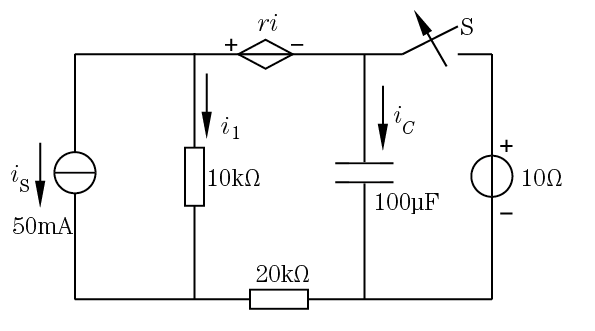
\includegraphics[width=1\textwidth]{p7-6-a.png}
\caption*{(a)}
\end{minipage}
\begin{minipage}[t]{0.413\textwidth}
\centering
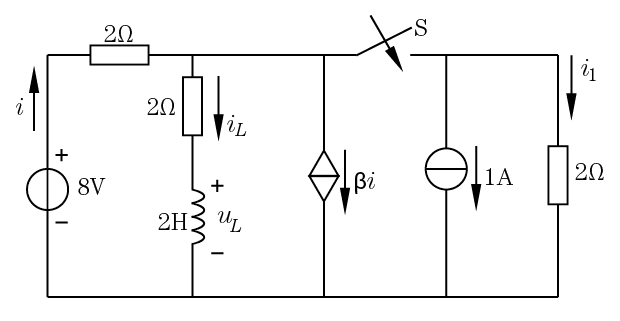
\includegraphics[width=1\textwidth]{p7-6-b.png}
\caption*{(b)}
\end{minipage}
\caption*{题图 7-6}
\end{figure}

\paragraph{解}

\begin{figure}[!htb]
\centering
\begin{minipage}[t]{0.321\textwidth}
\centering
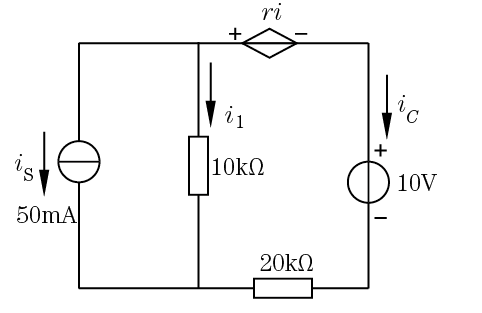
\includegraphics[width=1\textwidth]{p7-6-a-sol.png}
\caption*{(a)}
\end{minipage}
\begin{minipage}[t]{0.411\textwidth}
\centering
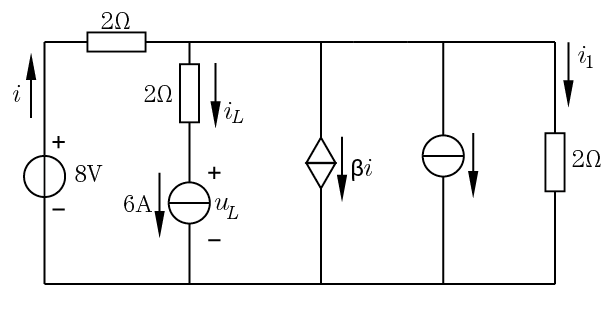
\includegraphics[width=1\textwidth]{p7-6-b-sol.png}
\caption*{(b)}
\end{minipage}
\caption*{图 7-6}
\end{figure}

(a) 换路前,$u_c=10\volt$

则换路后瞬间,如图 7-6 (a) 所示,
$$ 50i_1 + 10 = 10000i_1 + 20000(i_1+0.05) $$

得
$$i_1 = -0.033\ampere, i_C = -i_\source - i_1 = -0.017\ampere$$

(b) 换路前
\begin{align*}
\left\{ \begin{aligned}
8 &= 2i+2i_L \\
i &= i_L + 4i
\end{aligned} \right.
\end{align*}
$$\therefore i=-2 \ampere, i_L = 6\ampere $$

则换路后瞬间,如图 7-6 (b) 所示,
\begin{align*}
\left\{ \begin{aligned}
8 &= 2i + 2i_1 \\
i &= 6 + 4i + 1 + i_1
\end{aligned} \right.
\end{align*}
$$\therefore i = -5.5\ampere, i_1 = 9.5\ampere, i_L = 6\ampere, u_L = 8-2i-2i_L = 7\volt $$

\paragraph{7-10}\label{7-10}
题图 7-10 所示电路换路前已达稳态,$t=0$ 时开关 $\rm S$ 打开。求电容电压 $u_C(t)$,并定性画出其变化曲线。

\begin{figure}[!htb]
\centering
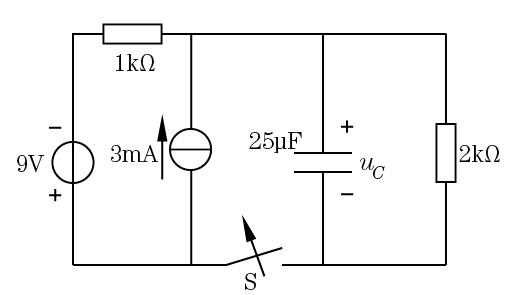
\includegraphics[width=0.351\textwidth]{p7-10.png}
\caption*{题图 7-10}
\end{figure}

\paragraph{解}
换路前
$$ 9 = -u_C + (3 - \frac{u_C}{2})$$
$$ \therefore u_C(0^-) = -4\volt = u_C(0^+) $$
$$ \tau = RC = 0.05 \second, u_C(+\infty) = 0 $$
$$ \therefore u_C(t) = -4 \E ^{-20t} \volt, t \ge 0 $$

图像如图 7-10 所示。

\begin{figure}[!htb]
\centering
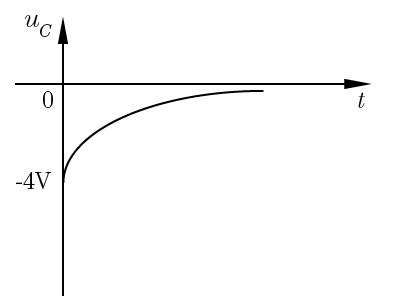
\includegraphics[width=0.262\textwidth]{p7-10-sol.png}
\caption*{图 7-10}
\end{figure}

\paragraph{7-11}\label{7-11}
题图 7-11 所示电路换路前已达稳态,$t=0$ 时开关 $\rm S$ 闭合。求流过电感的电流 $i_L(t)$,并定性画出其变化曲线。

\begin{figure}[!htb]
\centering
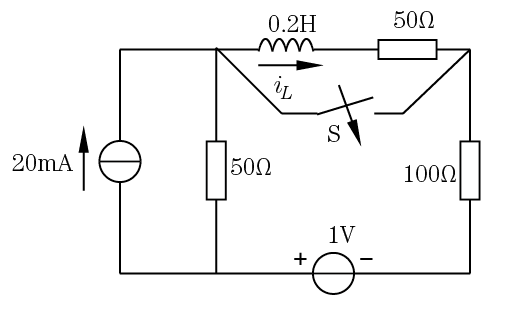
\includegraphics[width=0.340\textwidth]{p7-11.png}
\caption*{题图 7-11}
\end{figure}

\paragraph{解}
换路前
$$ 1 = (i_L - 0.02) \times 50 + 50 i_L + 100 i_L $$
$$ \therefore i_L(0^-) = 0.01\ampere = i_L(0^+) $$
$$ \tau = L/R = 0.2\henry / 50\ohm = 0.004\second, i_L(+\infty) = 0 $$
$$ \therefore i_L(t) = 0.01 \E ^{-250t} \ampere, t \ge 0 $$

图像如图 7-11 所示。

\begin{figure}[!htb]
\centering
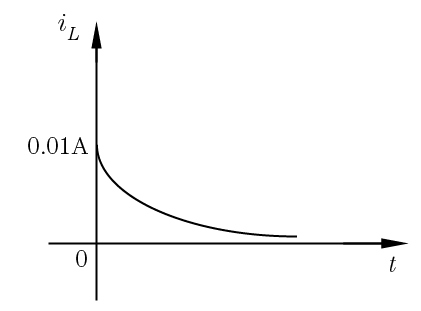
\includegraphics[width=0.281\textwidth]{p7-11-sol.png}
\caption*{图 7-11}
\end{figure}

\paragraph{7-23}\label{7-23}
题图 7-23 所示电路 $t=0$ 时闭合开关 $S$。求 $i_C$ 的零状态响应、零输入响应和全响应。

\begin{figure}[!htb]
\centering
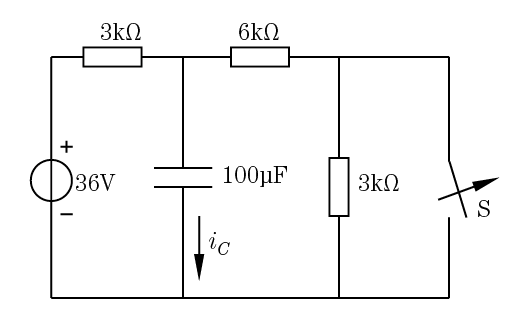
\includegraphics[width=0.349\textwidth]{p7-23.png}
\caption*{题图 7-23}
\end{figure}

\paragraph{解}
从$C$看入的等效电阻为$R = 3\kiloohm // 6\kiloohm = 2\kiloohm$, 则时间常数 $\tau = RC = 0.2\second$

1) 零状态响应
$$u_{C \rm zs}(+\infty) = \frac{36}{3+6} \times 6 = 24\volt$$
$$\therefore u_{C \rm zs}(t) = 24(1-\E ^{-5t})\volt $$
$$ i_{C \rm zs}(t) = C\cdot \frac{\D u_{C \rm zs}}{\D t} = 12 \E ^{-5t} \milliampere$$

2) 零输入相应
$$u_{C \rm zi}(0^+) = 27\volt$$
$$\therefore u_{C \rm zi}(t) = 27\E ^{-5t}\volt $$
$$ i_{C \rm zi}(t) = C\cdot \frac{\D u_{C \rm zi}}{\D t} = -13.5 \E ^{-5t} \milliampere$$

则全响应
$$i(t) = i_{C \rm zs}(t)+i_{C \rm zi}(t) = -1.5 \E ^{-5t} \milliampere$$

\end{document} 